\noindent

\includegraphics[height=1.25cm]{images/pictograms/tools}

%%%%%%%%%%%%%%%%%%%%%%%%%%%%%%%%%%%%%%%%%%%%%%%%%%%%%%%%%%%%%%%%%%%%%%%%%%%%%%%%%%%%%%%%%%%%%%%%%%%

\begin{flushright} {\tiny {\color{gray} python\_codes/fieldstone\_56/text.tex}} \end{flushright}


\par\noindent\rule{\textwidth}{0.4pt}

\begin{center}
\inpython
{\small Code: \url{https://github.com/cedrict/fieldstone/tree/master/python_codes/fieldstone_56}}
\end{center}

\par\noindent\rule{\textwidth}{0.4pt}

{\sl This stone was developed in collaboration with A. Hendrickx}. \index{contributors}{A. Hendrickx}

\par\noindent\rule{\textwidth}{0.4pt}

{\bf \color{teal} Purpose}: provide an implementation of the diamond-square algorithm.

\par\noindent\rule{\textwidth}{0.4pt}

%%%%%%%%%%%%%%%%%%%%%%%%%%%%%%%%%%%%%%%%%%%%%%%%%%%%%%%%%%%%%%%%%%%%%%%%%%%%%%%%%%%%%%%%%%%%%%%%%%%

According to Wikipedia\footnote{\url{https://en.wikipedia.org/wiki/Diamond-square_algorithm}}:
``The diamond-square algorithm is a method for generating heightmaps for computer graphics. It is a slightly better algorithm than the three-dimensional implementation of the midpoint displacement algorithm, which produces two-dimensional landscapes. It is also known as the random midpoint displacement fractal, the cloud fractal or the plasma fractal, because of the plasma effect produced when applied. 

The diamond-square algorithm starts with a two-dimensional grid, then randomly generates terrain height from four seed values arranged in a grid of points so that the entire plane is covered in squares.''

The idea was first introduced by \textcite{fofc82} at SIGGRAPH\footnote{
SIGGRAPH (Special Interest Group on Computer Graphics and Interactive Techniques) is an annual conference centered around computer graphics organized by ACM, starting in 1974.} in 1982.


The function\footnote{\url{https://github.com/AgnesHendrickx/MTE/blob/main/art_DEM.py}}
 {\tt generate\_fractal\_map} is taken from the MTE code\footnote{\url{https://mte.readthedocs.io/en/latest/}}. That function was 100\% written by Agnes.

This specific implementation of the diamond-square algorithm also adds some diffusion to the resulting surface by 
means of the {\tt gaussian\_filter} function from the {\tt scipy.ndimage} module. It is controlled
by the {\tt sigma} parameter\footnote{\url{https://docs.scipy.org/doc/scipy/reference/generated/scipy.ndimage.gaussian_filter.html}}.

This algorithm only works on a square surface of size $L\times L$
discretised by means of a $N_x \times N_y$ grid where 
$N_x=N_y=2^{size}+1$. For example if $size=8$ then the grid counts 
$257\times 257$ nodes.
The {\tt roughness} parameter determines the amplitude of the generated 
topography. 

\begin{center}
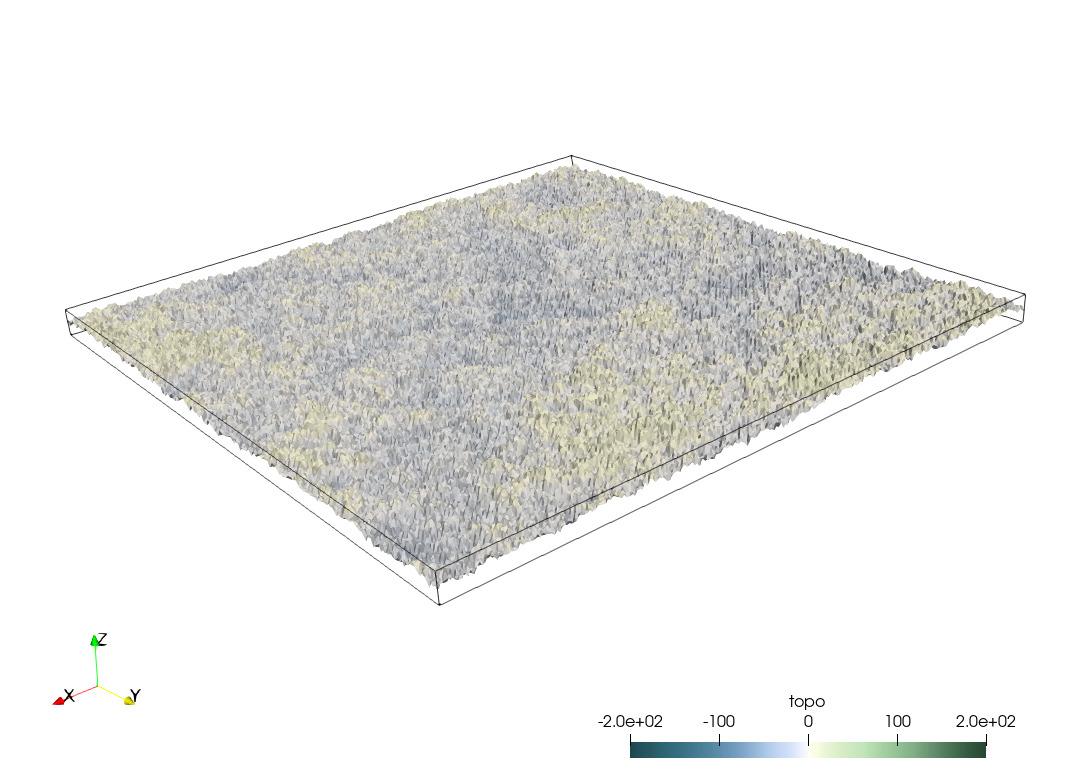
\includegraphics[width=5.7cm]{python_codes/fieldstone_56/results/topo010_3d}
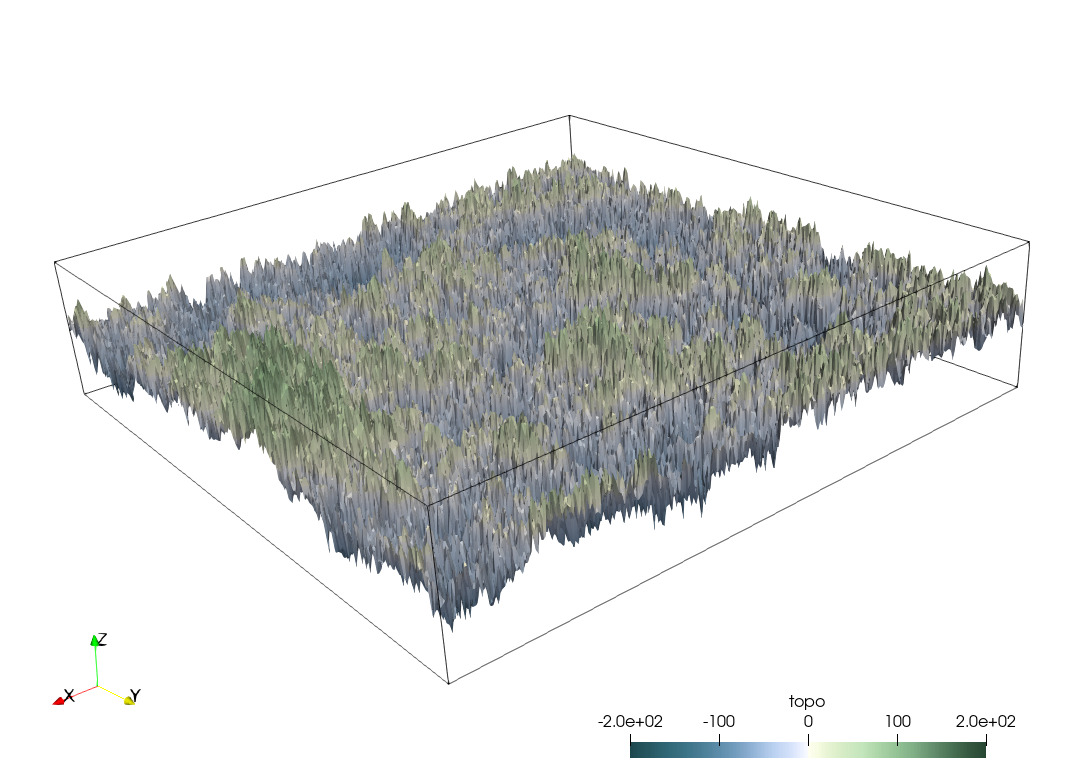
\includegraphics[width=5.7cm]{python_codes/fieldstone_56/results/topo050_3d}
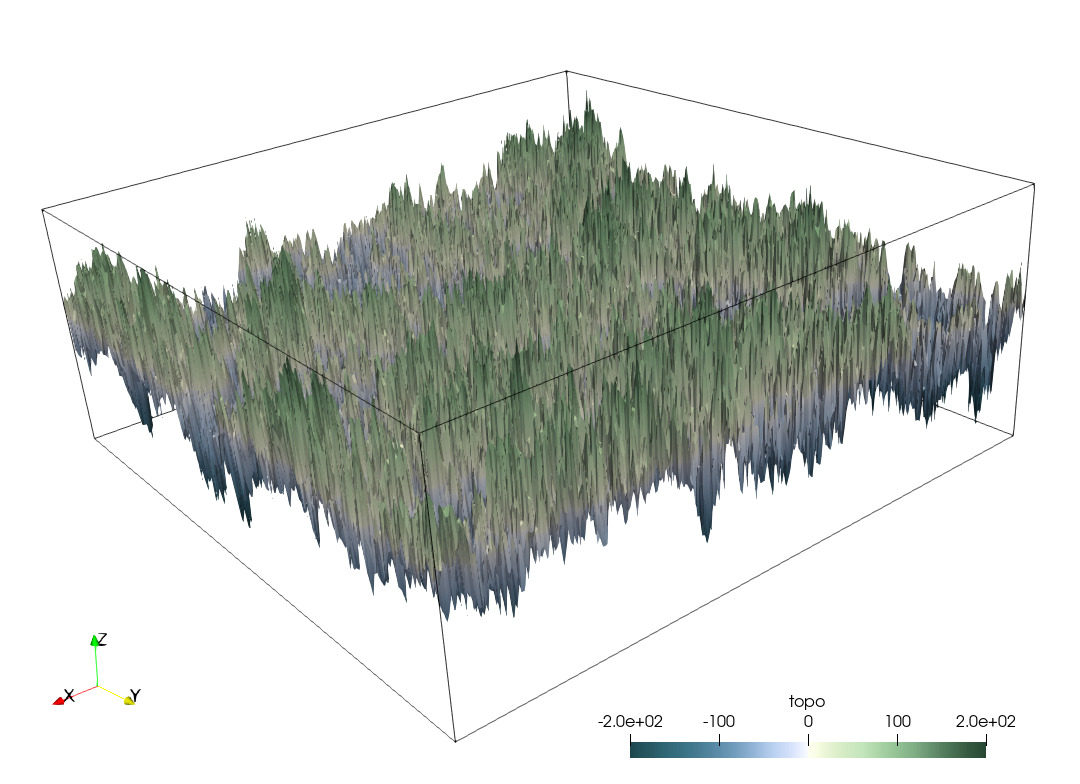
\includegraphics[width=5.7cm]{python_codes/fieldstone_56/results/topo100_3d}\\
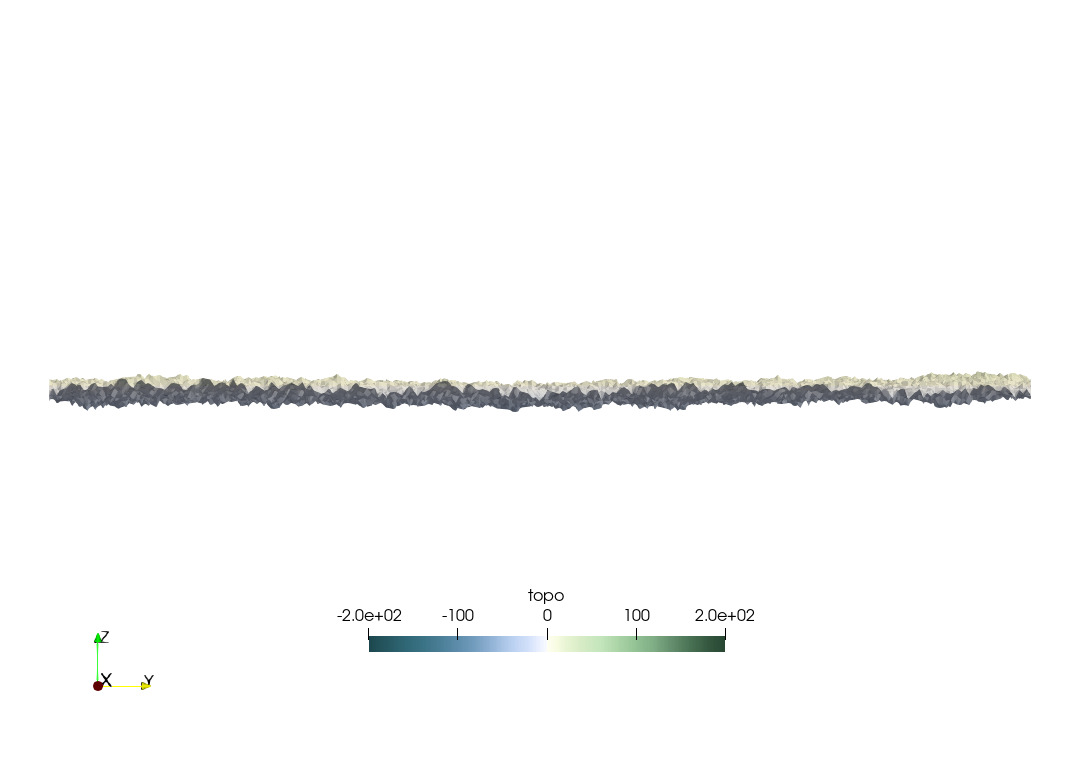
\includegraphics[width=5.7cm]{python_codes/fieldstone_56/results/topo010}
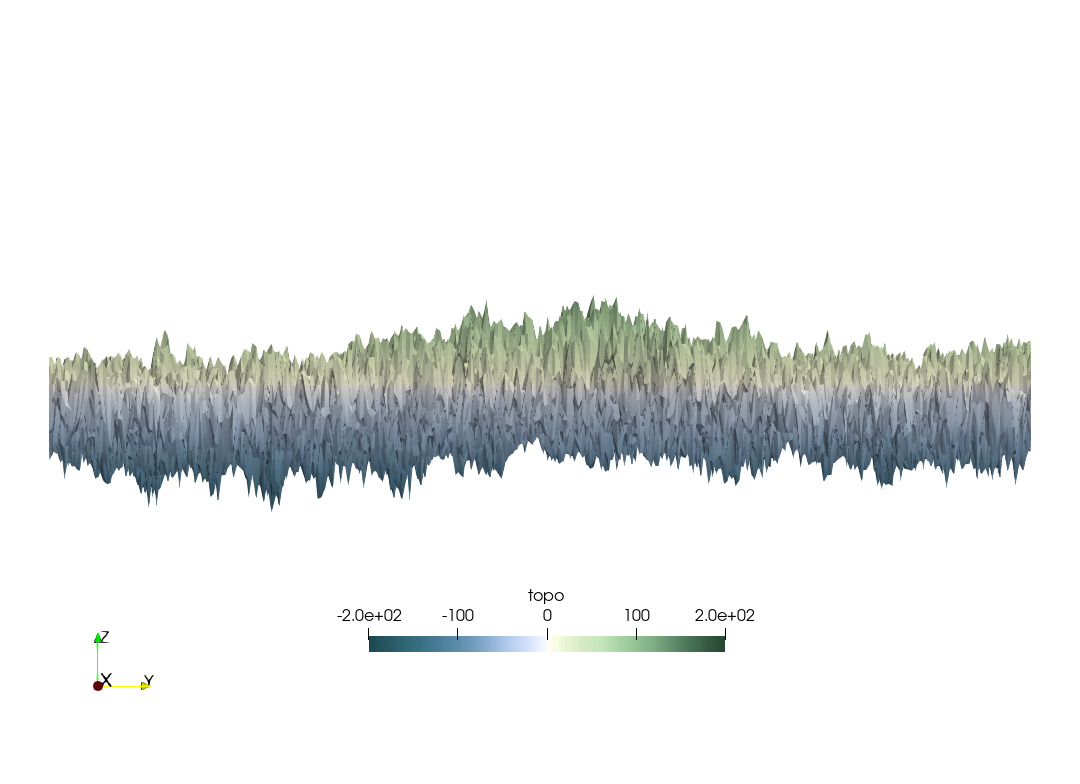
\includegraphics[width=5.7cm]{python_codes/fieldstone_56/results/topo050}
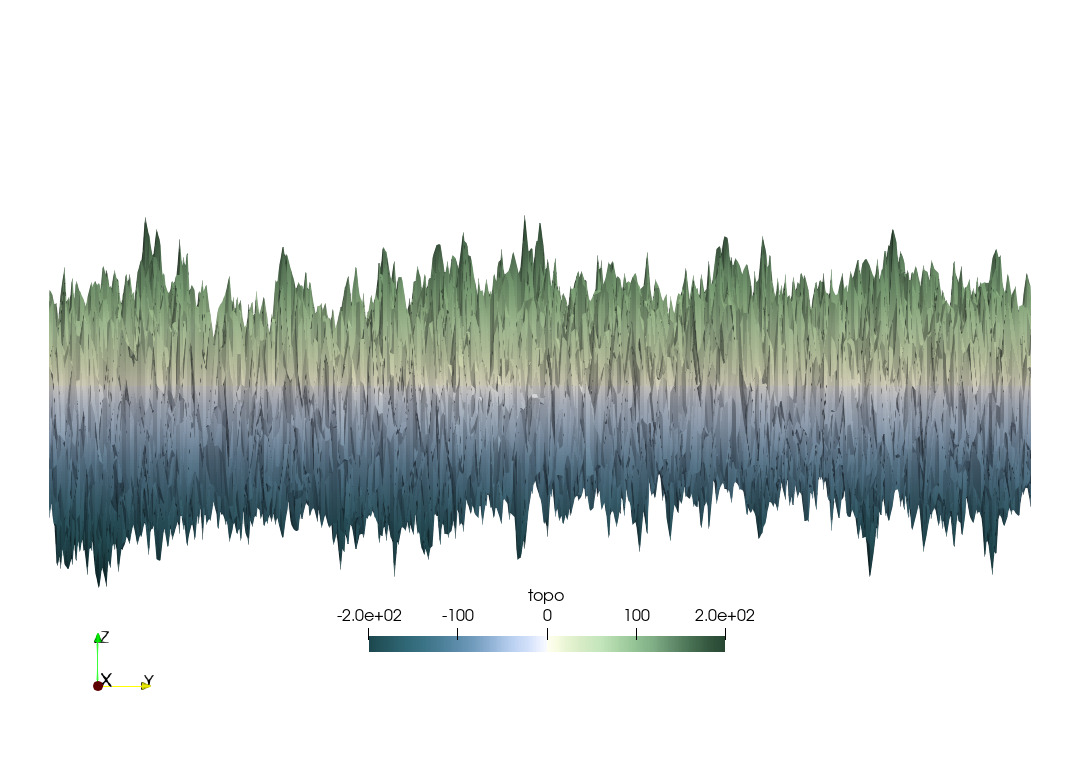
\includegraphics[width=5.7cm]{python_codes/fieldstone_56/results/topo100}\\
{\captionfont Resulting topography for $L=1000$m, grid 257x257, $\sigma=0$ and for 
roughness=10,50,100 from left to right.}
\end{center}

\begin{center}
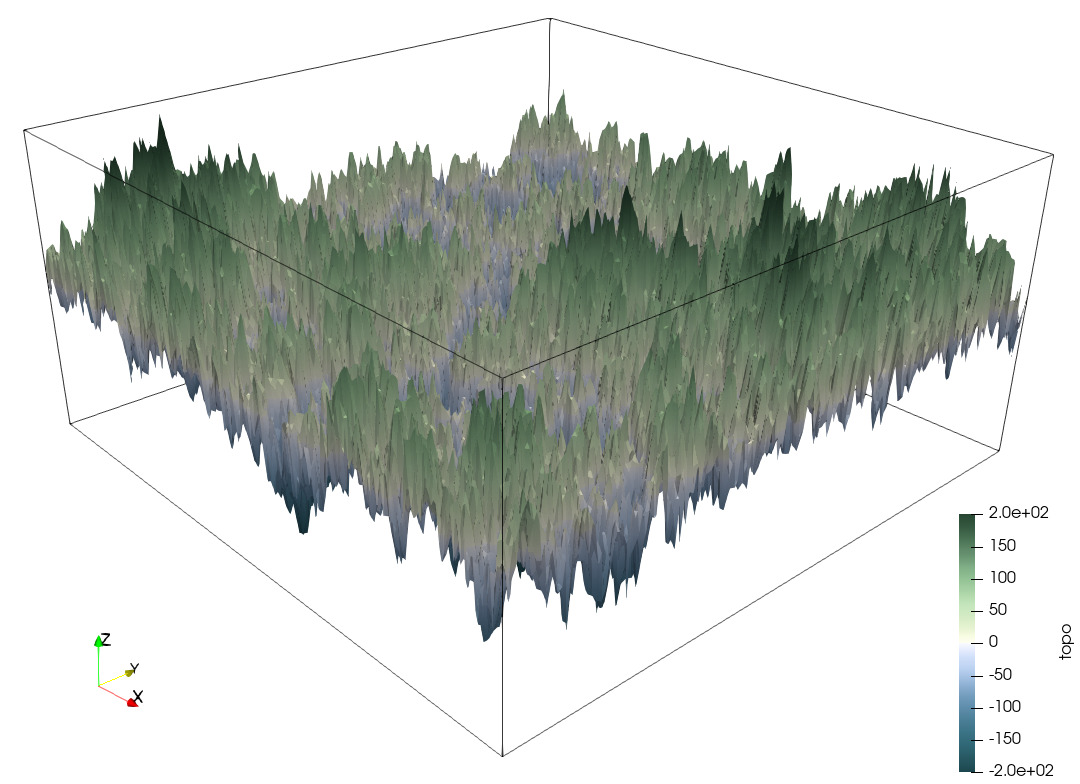
\includegraphics[width=7cm]{python_codes/fieldstone_56/results/topo_sig000}
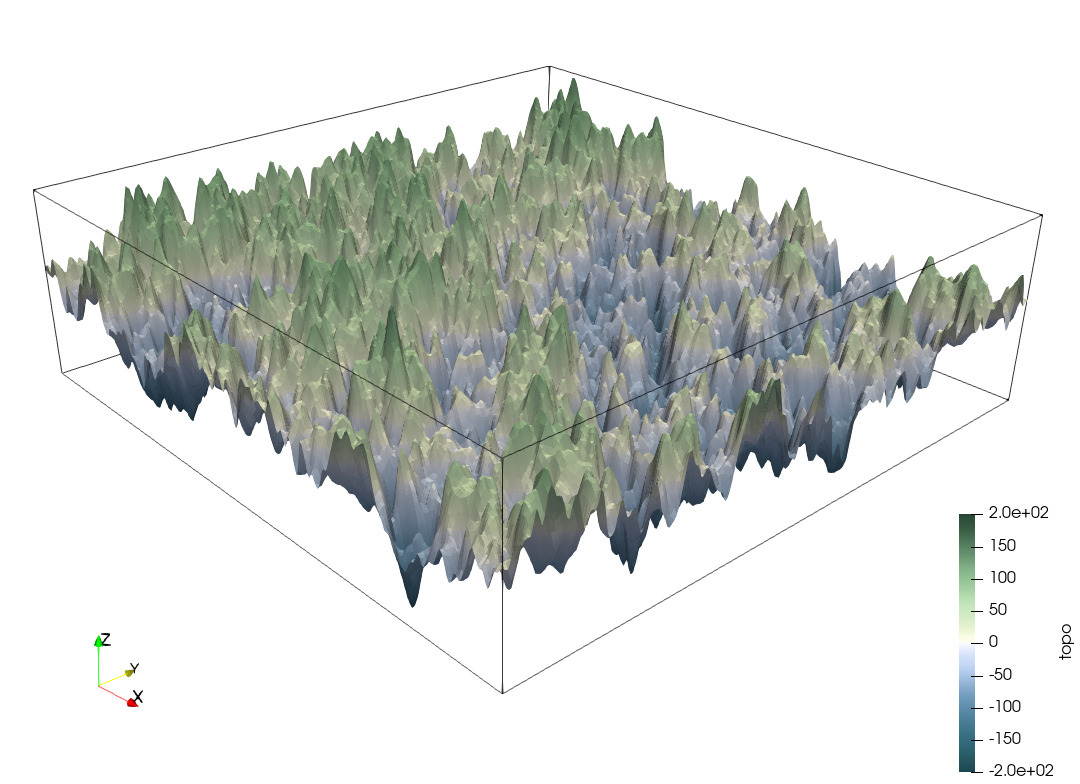
\includegraphics[width=7cm]{python_codes/fieldstone_56/results/topo_sig001}\\
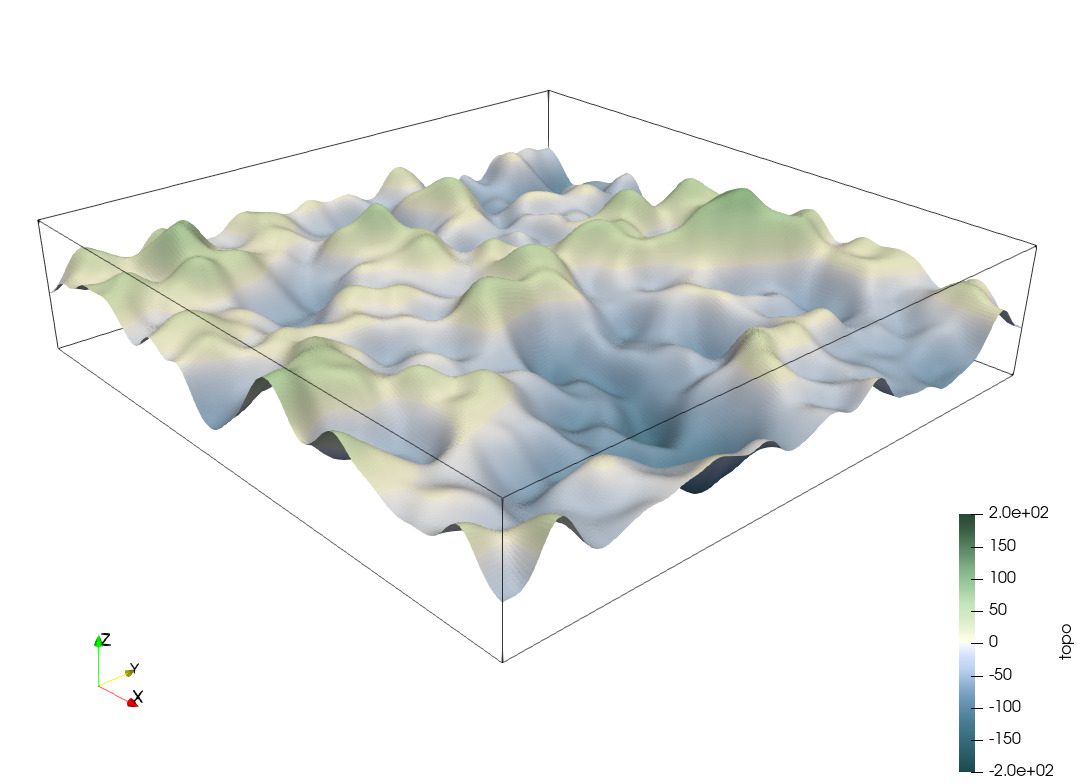
\includegraphics[width=7cm]{python_codes/fieldstone_56/results/topo_sig005}
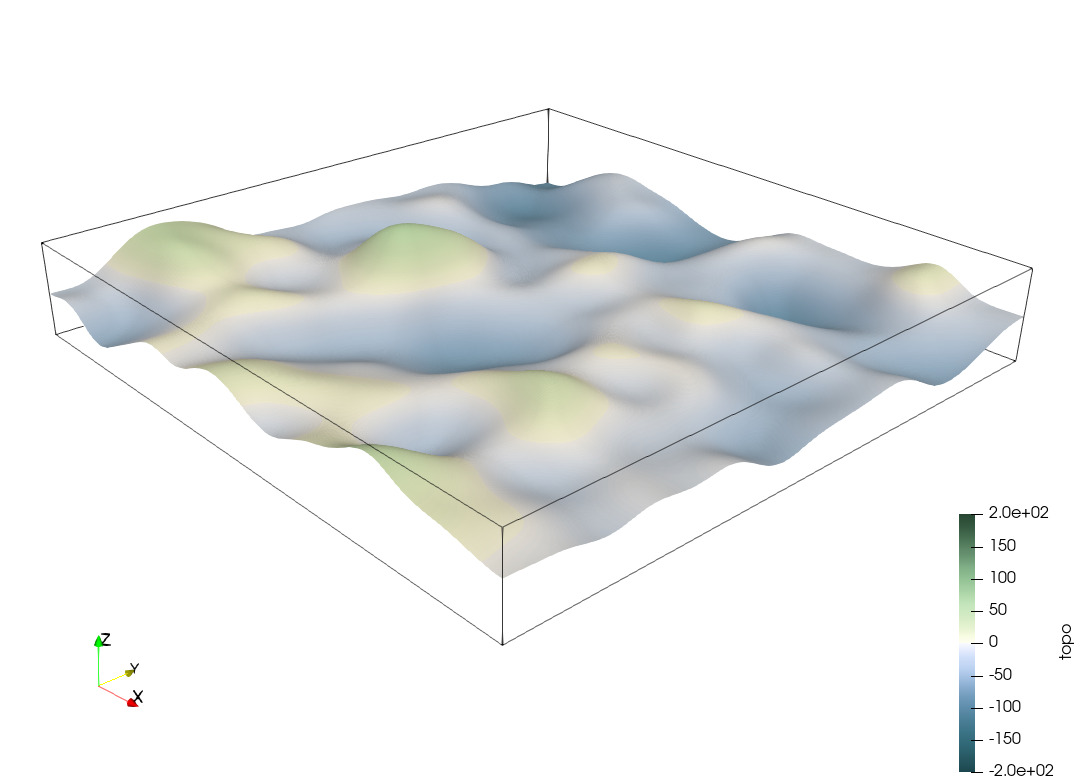
\includegraphics[width=7cm]{python_codes/fieldstone_56/results/topo_sig010}\\
{\captionfont Resulting topography for $L=1000$m, grid 257x257, 
roughness=100 and $\sigma=0,1,5,10$.}
\end{center}

